\begin{frame}{Ý nghĩa của phương trình vi phân trong bài toán chuyển động}
    %Dẫn từ phương trình vi phân => cần phép toán nguyên hàm và tích phân.

    %y'=f(x) =? y(x) = ?

    %Nguyên hàm, xác định hằng số C

    %Chúng ta đã biết về phép đạo hàm, nhưng có phép nào làm ngược lại quá trình không?
    \begin{center}
    \begin{minipage}{0.45\linewidth}
    \begin{figure}
        \centering
        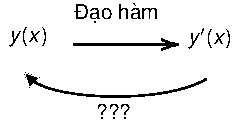
\includegraphics[width=0.6\linewidth]{Figures/Int_1.pdf}
        \label{fig:Int_1}
    \end{figure}
    \end{minipage}
    \hspace{1mm}
    \begin{minipage}{0.4\linewidth}
        Giải phương trình vi phân
        \begin{equation*}
            y'(x) = f(x).
        \end{equation*}
    Sử dụng 
    \vspace{-2mm}
    
    \begin{equation*}
        dy = f(x) dx.
    \end{equation*}
    \end{minipage}
    \end{center}
    Ta định nghĩa một phép toán ngược quá trình đạo hàm. Ký hiệu là \("\displaystyle \int "\). Sao cho
    \vspace{1mm}
    
    \begin{equation}
        \int f(x) dx = y(x) + C \ \ \ \ \text{,Với \(C\) là hằng số}.
        \label{eq:int_1}
    \end{equation}
    
    Ta gọi phép toán ở (\ref{eq:int_1}) là nguyên hàm.
\end{frame}

\begin{frame}{Bài toán diện tích và phương pháp vét cạn}
\begin{center}
    \begin{minipage}{0.45 \linewidth}
        \begin{figure}
            \centering
            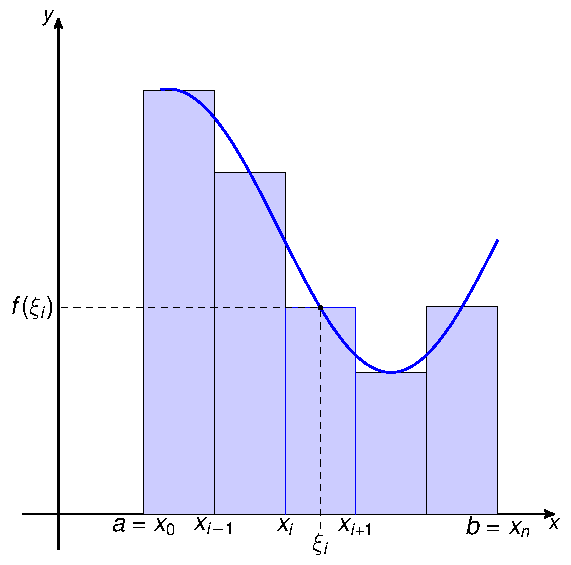
\includegraphics[width=1\linewidth]{Figures/Int_2.pdf}
            \label{fig:Int_2}
        \end{figure}
    \end{minipage}
    \begin{minipage}{0.45\linewidth}
        \begin{figure}
            \centering
            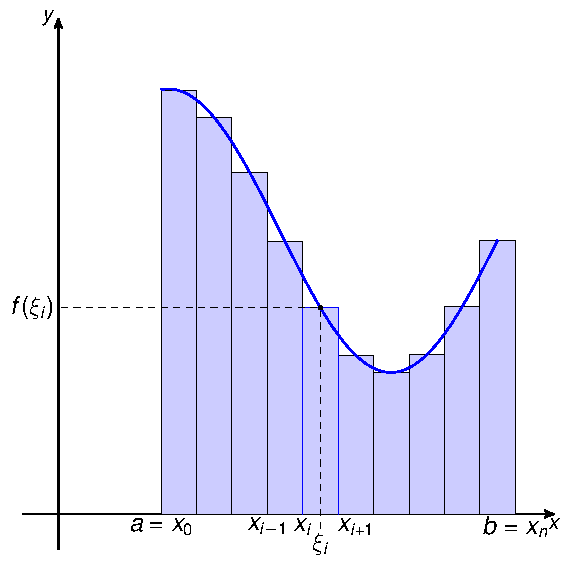
\includegraphics[width=1\linewidth]{Figures/Int_3.pdf}
            \label{fig:Int_3}
        \end{figure}   
    \end{minipage}
\end{center}

\end{frame}
\begin{frame}{Bài toán diện tích và phương pháp vét cạn}
    \begin{center}
        \begin{minipage}{0.4\linewidth}
        \begin{figure}
            \centering
            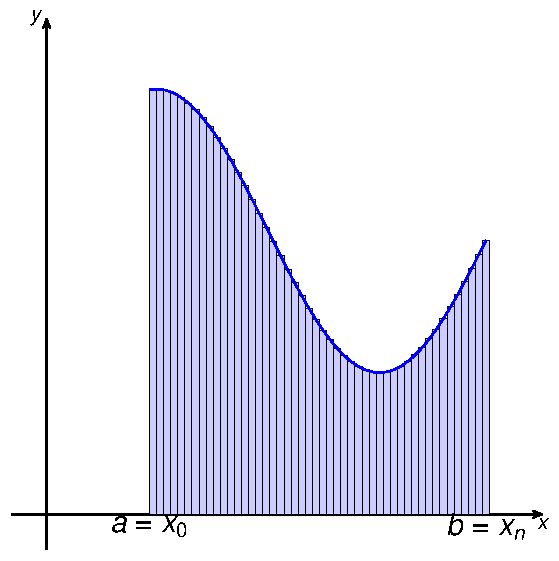
\includegraphics[width=1\linewidth]{Figures/Int_4.pdf}
            \caption{Khi ta chia đủ nhỏ}
            \label{fig:Int_4}
        \end{figure}
        \end{minipage}
        \hspace{1mm}
        \begin{minipage}{0.4\linewidth}
            Diện tích 
            \begin{equation}
            \label{eq:int_2}
            \begin{split}
                &S \simeq  \sum_{i=0}^n f(\xi_i) \Delta x \\
                &\text{Với}
                \left\{
                \begin{array}{ccc}
                \Delta x &=& x_{i+1} - x_i \\
                \xi_i &\in& [x_i,x_{i+1}]
                \end{array}
                \right.
            \end{split}
            \end{equation}  
            Đây là công thức tổng Riemann để xấp xỉ diện tích bên dưới đồ thị.
        \end{minipage}
    \end{center}
\end{frame}
\begin{frame}{Mối liên hệ nguyên hàm - tích phân}
    Ở công thức (\ref{eq:int_2}), ta có thể chọn tuỳ ý \(\xi_i\). Nên ta chọn \(\xi_i = x_i\). Lúc này
    \begin{equation*}
        S \simeq \sum_{i=0}^n f(x_i) \Delta x.   
    \end{equation*}
    Nếu ta lấy giới hạn sao cho các cột diện tích đủ nhỏ thì ta sẽ có
    \begin{equation}
        \displaystyle
        \Delta x \rightarrow dx \ \text{thì} \ \sum_{i=0}^n \rightarrow \int_{a}^b
        \label{eq:int_3}
    \end{equation}
\end{frame}
\begin{frame}{Ví dụ}
    Cho một vật di chuyển với đồ thị vận tốc \(v = f(t) = at+b\). Tìm quãng đường nó di chuyển được trong thời gian \(t \in [c,d]\). Tìm diện tích trong khoảng \(t \in [c,d]\).
    \begin{center}
                    \underline{Giải}
    \end{center}
    \begin{center}
        \begin{minipage}{0.35\linewidth}
            \begin{figure}
                \centering
                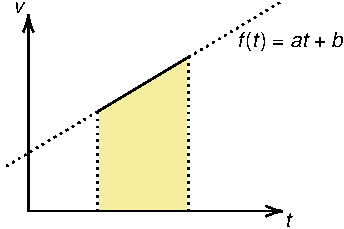
\includegraphics[width=1\linewidth]{Figures/Int_5.pdf}
                \label{fig:Int_5}
            \end{figure}
        \end{minipage}
        \hspace{1mm}
        \begin{minipage}{0.5\linewidth}

            Quãng đường: 
            \begin{equation*}
                \Delta x = \int_{c}^{d} f(t) dt = \frac{a}{2} (d^2-c^2) + b(d-c).
            \end{equation*}
            Diện tích: Đây là diện tích hình thang vuông.
            \begin{equation*}
            \begin{split}
                \Delta S &= \frac12 \left(f(d) + f(c)\right) (d-c) \\&=  \frac{a}{2} (d^2-c^2) + b(d-c).             
            \end{split}
            \end{equation*}
        \end{minipage}
    \end{center}
\end{frame}
\begin{frame}{Nguyên hàm và tích phân, định lý Leibniz–Newton}


    Định lý Leibniz–Newton

    \begin{mdframed}[backgroundcolor=BlueDefault!10, linecolor=BlueDefault, linewidth=1pt]
    Nếu nguyên hàm của \(f(x)\) là \(F(x)\) thì 
    \begin{equation}
        \int_{a}^{b} f(x) dx = F(b) - F(a).      
    \end{equation}
    \end{mdframed}
    

    
\end{frame}

\begin{frame}{Giải phương trình vi phân: phân ly biến số}
    Phương pháp phân ly biến số dùng để giải quyết các phương trình vi phân cơ bản.
    \begin{equation*}
        f(x,y,y') = 0 .
    \end{equation*}
    Tách biến có nghĩa là mỗi vế của phương trình sẽ chỉ chứa một biến
    \begin{equation}
        f(x,y,y') = 0  \longrightarrow h(y) y' = g(x) \Longrightarrow{h(y) dy = g(x) dx}
    \end{equation}
    Ví dụ: Cho phương trình vi phân


    \begin{center}
        \begin{minipage}{0.45\linewidth}
            \begin{equation*}
                \begin{array}{ccl}
                &\displaystyle \frac{dv}{dt} &= -bv \\
                \pause 
                \\
                \Longrightarrow &\displaystyle \frac{dv}{v} &= -b dt \\
                \end{array} 
            \end{equation*}
        \end{minipage}
        \hspace{1mm}
        \begin{minipage}{0.5\linewidth}
            \begin{equation*}
                \begin{array}{ccl}
                \Longrightarrow &\displaystyle \int_{v_0}^{v(t)} \frac{dv}{v} &=\displaystyle  -\int_{0}^{t} b dt \\
                \\
                \Longrightarrow & \ln (v(t)/v_0)  &= -bt \\
                \end{array}  
            \end{equation*}
        \end{minipage}
    \end{center}
\end{frame}